\chapter{Konfiguracja projektu}
\label{cha:vivado-conf}

%TODO Kiepski tytuł dla rodziąłu - mało mówi o jego treści.
%TODO Dla całego rodziału - za krótkie akapity

Użycie funkcjonalności opisywanych w niniejszej pracy wymaga przeprowadzenia konfiguracji wykorzystywanych modułów logicznych oraz systemu operacyjnego. 
W poniższych podrozdziałach zebrano informacje związane z poruszanymi zagadnieniami. %TODO bardziej konkretnnie

\section{Podstawowa konfiguracja projektu}

Wykorzystany w projekcie układ -- Digilent ZYBO -- nie jest bezpośrednio wspierany przez środowisko Vivado. %TODO karta
Wynika z tego konieczność sprecyzowania parametrów układu na etapie tworzenia projektu. 
W trakcie modyfikowania projektu, w przypadku dodania modułów wykorzystujących interfejs wejścia/wyjścia, konieczna jest również konfiguracja parametrów interfejsu. 
Aby uprościć proces projektowania, zalecane jest skonfigurowanie obsługi układu przed utworzeniem projektu. 
Proces ten opisano w dokumentacji producenta \cite{zybo-in-vivado}.

\subsection{Vivado}
\label{sec:vivado-conf}
Utworzyć należy projektu typu \emph{,,RTL Project''}, z odznaczoną opcją \emph{,,Do not specify sources at this time''}.

W kroku \emph{,,Add Constraints''} dodać należy plik konfiguracyjny dla wybranego układu. 
W przypadku ZYBO, plik ten jest dostępny na stronie producenta. 
W kolejnym kroku możliwe jest skonfigurowanie parametrów układu. 
Wykorzystać do tego należy zakładkę \emph{,,Boards''} i wybrać wykorzystywany model.

Po utworzeniu projektu, skonfigurować należy właściwą przestrzeń roboczą dla projektu, wykorzystując do tego opcję \emph{,,IP Integrator --> Create Block Design''}.

Do nowo utworzonej przestrzeni dodać należy moduł IP reprezentujący procesor ZYNQ -- \emph{,,ZYNQ7 Processing System''}.

W kolejnych krokach należy dokonać konfiguracji modułu procesora, klikając dwukrotnie na moduł.

\begin{itemize}
	\item Kanały interfejsu AXI mogą być konfigurowane przez zakładkę \emph{,,PS-PL Configuration''}. Możliwa jest aktywacja kanałów ogólnego przeznaczenia (\emph{GP}) oraz wysokiej wydajności (\emph{HP}).
	
	\item Interfejsy komunikacji konfigurowane mogą być z poziomu zakładki \emph{,,MIO Configuration''}. Zalecane jest aktywowanie interfejsów \emph{ENET 0}, \emph{SD 0} i \emph{UART 1} ze względu na ich wykorzystanie na dalszym etapie pracy.
	
	Przykład konfiguracji interfejsów wejścia/wyjścia przedstawiono na rysunku \ref{fig:vivado-mio-configuration}.
	\begin{figure}[ht]
		\centering
		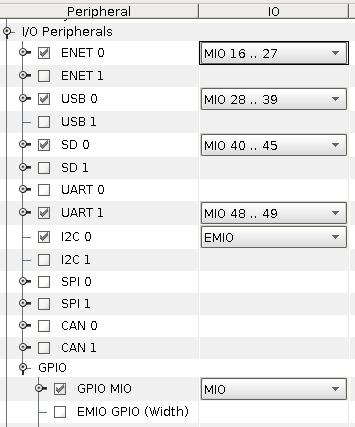
\includegraphics[height=8cm]{img/vivado/mio-configuration.png}
		\caption{Okno konfiguracji interfejsów wejścia i wyjścia.}
		\label{fig:vivado-mio-configuration}
	\end{figure}
	
	\item Parametry sygnałów zegarowych dostępnych z poziomu układów logiki reprogramowalnej modyfikować można w zakładce \emph{,,Clock Configuration/PL Fabric Clocks''}.
	
	\item Częstotliwość pracy procesora oraz pamięci zmienić można w zakładce \emph{,,Clock Configuration/Processor/Memory Clocks''}.
	
	%TODO Jakie mają być te częstotliwości ?
\end{itemize}

Po ukończeniu etapu konfiguracji procesora i powrocie do głównego okna programu, należy użyć opcji \emph{,,Run Block Automation''}. 
Utworzone zostaną połączenia interfejsów pamięci \texttt{DDR} oraz \texttt{FIXED\_IO}.

W przypadku zdefiniowania interfejsów AXI, połączyć należy właściwe sygnały zegarowe. 
Przykład wynikowej konfiguracji projektu przedstawiono na rysunku \ref{fig:vivado-config-result}.

	\begin{figure}[ht]
		\centering
		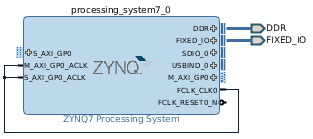
\includegraphics[]{img/vivado/vivado-config-result.png}
		\caption{Okno projektu.}
		\label{fig:vivado-config-result}
	\end{figure}
	
Przedstawiona konfiguracja stanowi podstawę każdego projektu wykorzystującego moduł procesora Zynq.

Po zakończeniu konfiguracji, wygenerować należy warstwę HDL, korzystając z opcji \emph{,,Create HDL Wrapper''} dostępnej po kliknięciu prawym przyciskiem myszy na utworzony wcześniej plik źródłowy.

Skonfigurowany w ten sposób projekt może być budowany i uruchamiany na platformie Zybo.

\subsection{SDK}

W celu utworzenia projektu aplikacji w SDK, konieczne jest wyeksportowanie plików opisujących projekt z poziomu Vivado, wykorzystując do tego opcję \emph{,,File/Export/Export Hardware''} z zaznaczoną opcją \emph{,,Include bitstream''}.

W efekcie, dostępna powinna być aplikacja \texttt{\textit{nazwa\_projektu}\_hw\_platform\_0}, zawierająca plik \texttt{nazwa\_projektu.hdf}. Aplikacja ta stanowi podstawę każdego budowanego programu \textit{bare-metal}. %TODO to jest aplikacja, czy konfiguracja sprzętowa ?

W przypadku budowania aplikacji na platformę PetaLinux, na etapie tworzenia projektu, zmodyfikować należy pole \emph{,,OS Platform''} na wartość \emph{,,linux''}, \emph{,,Processor Type''} na \emph{,,ps7\_cortexa9''} oraz wybrać właściwy język programowania.

W kontekście tak utworzonej aplikacji nie znajdują się biblioteki dostarczane przez firmę \emph{Xilinx}, wykorzystywane w aplikacjach \textit{bare-metal}, dostępna jest jednak pełna biblioteka języka \emph{C} oraz \emph{C++}.
%TODO zdanie niejasne

W celu uruchomienia aplikacji systemowej na platformie ZYBO, przeprowadzić należy proces budowania i skopiować wynikowy plik z katalogu \texttt{Debug} lub \texttt{Release} do systemu plików systemu PetaLinux. 
Wykorzystać można do tego narzędzie SSH:

\begin{lstlisting}[breaklines=true]
scp Debug/hello-world.elf root@adres-ip:~/
\end{lstlisting}

Aplikację uruchomić można przy użyciu konsoli użytkownika, również stosując narzędzie SSH.

\subsection{PetaLinux}
\label{sec:petalinux-config}

%TODO - a tu nie trzeba zrobić czegoś wcześniej ? Pobrać zainstalowć itp ?

Utworzenie struktury katalogów projektu wykonywane jest przy użyciu poniższego polecenia.

\begin{lstlisting}[breaklines=true]
petalinux-create -t project --template zynq --name (*@\textit{nazwa-projektu}@*)
cd (*@\textit{nazwa-projektu}@*)
\end{lstlisting}

Powstała struktura zintegrowana jest z systemem kontroli wersji \emph{git}, co pozwala utrzymać uporządkowanie danych wewnątrz projektu oraz wersjonowanie. 
Zarządzanie repozytorium wykorzystuje podstawowe komendy narzędzia. %TODO styl !

Kolejnym krokiem jest zaimportowanie projektu \emph{Vivado}.

\begin{lstlisting}[breaklines=true]
petalinux-config --get-hw-description=(*@\textit{/sciezka/do/projektu/projekt.sdk/}@*)
\end{lstlisting}

Jeśli polecenie wywołane zostało po raz pierwszy dla danego projektu, uruchomione zostanie narzędzie konfiguracyjne, domyślne ustawienia są jednak poprawne.

Konfiguracja projektu odbywa się przy użyciu polecenia \texttt{petalinux-config}.
Skonfigurować należy metodę uruchamiania systemu -- w omawianym przypadku, uruchomienie następuje na bazie plików znajdujących się na karcie SD.
\begin{lstlisting}[breaklines=true]
petalinux-config
Image Packaging Configuration -> Root filesystem type -> SD card
\end{lstlisting}

Należy również zmodyfikować argumenty przekazywane systemowi na etapie uruchamiania, umożliwiając wykorzystanie sterowników do modułów logiki reprogramowalnej.

\begin{lstlisting}[breaklines=true]
petalinux-config
Kernel Bootargs -> dezaktywować opcję Generate boot args automatically i zdefiniować własną wartość
console=ttyPS0,115200 earlyprintk uio_pdrv_genirq.of_id=generic-uio root=/dev/mmcblk0p2 rw rootwait 
\end{lstlisting}
Następnie, przeprowadzić należy proces budowania systemu oraz wygenerować pliki wynikowe.

\begin{lstlisting}[breaklines=true]
petalinux-build
petalinux-package --boot --fsbl images/linux/zynq_fsbl.elf --fpga images/linux/system_wrapper.bit --u-boot --force
petalinux-package --image -c rootfs --format initramfs
\end{lstlisting}

Uruchomienie systemu wymaga przygotowania karty SD -- musi ona posiadać dwie partycje, pierwszą, z etykietą \emph{boot} i systemem plików \emph{fat32}, drugą -- odpowiednio \emph{sys} i \emph{ext4}. 
Pierwsza z nich, zawierająca pliki wymagane na etapie inicjalizacji systemu, musi być poprzedzona 4 MB niezaalokowanej przestrzeni i mieć rozmiar co najmniej 40 MB. 
Druga partycja zawiera pliki systemowe, jej rozmiar powinien wynosić co najmniej kilkaset megabajtów. 
Proces formatowania przeprowadzić można przy użyciu narzędzia \emph{gparted}.
%TODO może screen z gparted jak to wygląda.

Pliki wynikowe należy przenieść na kartę SD, korzystając z poleceń.

\begin{lstlisting}[breaklines=true]
rm -rf /(*@\textit{punkt-montowania}@*)/sys/*
cp images/linux/BOOT.BIN /(*@\textit{punkt-montowania}@*)/boot/
cp images/linux/image.ub /(*@\textit{punkt-montowania}@*)/boot/
cp images/linux/rootfs.cpio /(*@\textit{punkt-montowania}@*)/sys/
cd /(*@\textit{punkt-montowania}@*)/
pax -rvf rootfs.cpio
sync
cd -
\end{lstlisting}

Ze względu na mechanizm buforowania przez kontroler operacji zapisu danych, pamiętać należy o wywołaniu polecenia \texttt{sync}, zapewniającego zachowanie integralności danych.

Karta SD pozwala na uruchomienie systemu operacyjnego na układzie i przechowywanie danych użytkownika pomiędzy startami układu. 
Dalsza praca z systemem odbywać się może przez protokoły komunikacji \emph{SSH} lub \emph{UART}.

\section{Konfiguracja modułu AXI DMA}
\label{sec:vivado-axi-dma}

%TODO 1-2 zdania wstępu

\subsection{Vivado}
Oprogramowanie Vivado umożliwia zbudowanie modułu wykorzystującego protokół AXI przez użycie opcji \emph{,,Create and package new IP...''}, zawartej w menu \emph{Tools}.

Na ekranie wyboru zadania wybrać należy opcję \emph{,,Create a new AXI4 peripheral''}.

Po zdefiniowaniu podstawowych danych związanych z modułem, takich jak jego nazwa i nazwisko autora, w kolejnym kroku możliwe będzie zdefiniowanie interfejsu modułu. 
Na tym etapie konfiguracji skonfigurować należy wszystkie połączenia wykorzystujące interfejs AXI. %TODO ????

W przypadku modułu konfiguracyjnego o podstawowej strukturze, interfejs zawierać powinien jedno połączenie wykorzystujące protokół AXI w wersji \emph{Lite}, działający w trybie \emph{slave}, z oczekiwaną liczbą rejestrów. 
Każdy rejestr powinien być związany z jedną wartością, której konfiguracja ma być możliwa. 
Przykład konfiguracji przedstawiono na rysunku \ref{fig:axi-dma-interfaces-conf}.
%TODO jest Pan pewnien, że taki moduł to DMA ?

\begin{figure}[h]
	\centering
	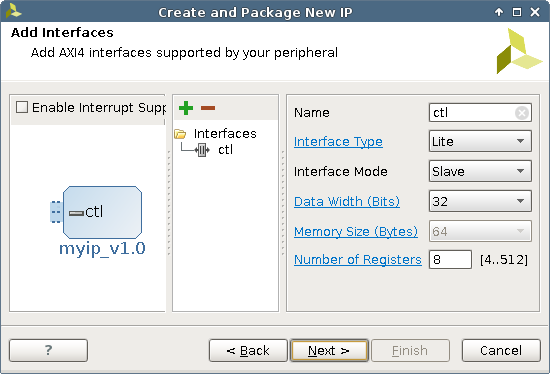
\includegraphics[width=8cm]{img/vivado/axi-dma-interfaces-conf.png}
	\caption{Konfiguracja interfejsów modułu AXI DMA.}
	\label{fig:axi-dma-interfaces-conf}
\end{figure}

W omawianym przykładzie zdefiniowano interfejs AXI o nazwie \emph{ctl}, związany z ośmioma rejestrami o długości trzydziestu dwóch bitów w pamięci.

Zdefiniowanie interfejsów kończy proces podstawowej konfiguracji modułu. W kolejnym kroku należy wybrać opcję \emph{,,Edit IP''} w celu dostosowania kodu źródłowego modułu.

Po wygenerowaniu, z modułem powinien być związany jeden plik źródłowy, zwierający instrukcje odpowiadające za obsługę komunikacji przy użyciu interfejsu AXI.

Do pliku dodać należy elementy odpowiedzialne za zdefiniowanie wyjść modułu oraz przypisanie im właściwych wartości.

W celu zdefiniowania wyjść modułu, odpowiadające im wpisy należy umieścić po komentarzu \emph{,,// Users to add ports here''}. Przykład przedstawiono na listingu \ref{listing:axi-dma-outputs}. %TODO powt. zdefinowane

\begin{lstlisting}[breaklines, label=listing:axi-dma-outputs, caption=Definicja interfejsów wyjściowych modułu.]
// Users to add ports here
output wire parameter_a,
output wire [7:0] parameter_b,
output wire [15:0] parameter_c,
output wire [31:0] parameter_d,
// User ports ends
\end{lstlisting}

Zdefiniowano cztery sygnały wyjściowe, o różnej liczbie bitów.

Następnie, należy dokonać modyfikacji kodu odpowiedzialnego za powiązanie wartości parametrów z rejestrami modułu. 
Rejestry AXI zdefiniowane są poniżej linii \emph{,,//-- Number of Slave Registers N''}, gdzie \emph{N} to liczba dostępnych rejestrów. Rejestry te mają nazwy \texttt{slv\_reg\emph{n}}, gdzie \emph{n} to indeks rejestru -- nie jest zalecana modyfikacja tych nazw.

Modyfikacji kodu należy dokonać poniżej linii \emph{,,// Add user logic here''}. 
Przykład przedstawiono na listingu \ref{listing:axi-dma-associate}.

\begin{lstlisting}[breaklines, label=listing:axi-dma-associate, caption=Powiązanie wyjść z rejestrami modułu.]
// Add user logic here
assign parameter_a = slv_reg0[0];
assign parameter_b = slv_reg1[7:0];
assign parameter_c = slv_reg2[15:0];
assign parameter_d = slv_reg3[31:0];
// User logic ends
\end{lstlisting}

W przedstawionym przykładzie powiązano wartości parametrów bezpośrednio z danymi znajdującymi się w rejestrach. %TODO powt. przed
W rozbudowanych aplikacjach może być konieczne dodanie instrukcji modyfikujących wartości rejestrów przed przesłaniem ich na wyjście modułu.

Po ukończeniu modyfikacji modułu, konieczne jest zapisanie zmian i wygenerowanie plików wynikowych. 
W tym celu należy wykorzystać okno \emph{,,Package IP''}, sekcję \emph{,,Review and Package''}. 
Widok okna przedstawiono na rysunku \ref{fig:axi-dma-review-package}.

\begin{figure}[ht]
	\centering
	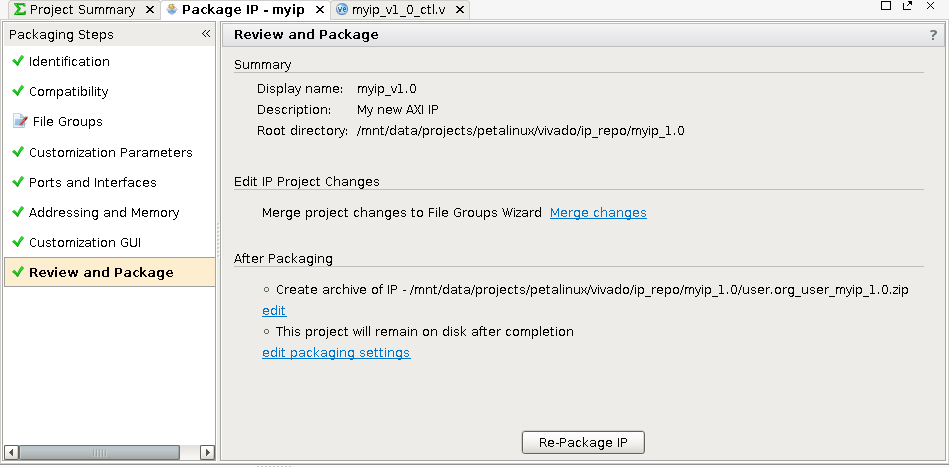
\includegraphics[width=12cm]{img/vivado/axi-dma-review-package.png}
	\caption{Okno finalizacji modyfikacji modułu.}
	\label{fig:axi-dma-review-package}
\end{figure}

Należy wybrać opcję \emph{,,Merge changes''}, umożliwiającą zintegrowanie wprowadzonych zmian z projektem bazowym. 
Następnie, można zakończyć edycję projektu przez wybór opcji \emph{,,Re-Package IP''}. 
Moduł będzie dostępny z poziomu interfejsu wyszukiwania modułów IP.

\subsection{SDK}
\label{sec:vivado-axi-dma-sdk}

Konfiguracja wartości parametrów modułu opiera się na zapisie do właściwych sektorów pamięci. %TODO nie lepiej pod właściwy adres w pamięci ?
W przypadku pracy w trybie \textit{bare-metal}, wykorzystać można instrukcję \emph{Xil\_Out32} z biblioteki \emph{xil\_io.h}. 
W przypadku pracy z systemem PetaLinux, wykorzystać należy biblioteki systemowe. 
Implementację\textit{ bare-metal} przedstawiono na listingu \ref{lis:axi-dma-bare-metal}, natomiast systemową na listingach \ref{lis:axi-dma-petalinux-main}, \ref{lis:axi-dma-petalinux-axi-h} i \ref{lis:axi-dma-petalinux-axi-c}.

\begin{lstlisting}[breaklines, language=C, label=lis:axi-dma-bare-metal, caption=Obsługa modułu w trybie bare-metal.]
#include "xparameters.h"
#include "platform.h"
#include "xil_io.h"

#define PARAMETER_A_REGISTER 0
#define PARAMETER_B_REGISTER 4
#define PARAMETER_C_REGISTER 8
#define PARAMETER_D_REGISTER 12

#define BASEADDR XPAR_ALGORITHM_PARAMETERS_0_CTL_BASEADDR

int main()
{
	init_platform();
	
	Xil_Out32(BASEADDR + PARAMETER_A_REGISTER, 1);
	Xil_Out32(BASEADDR + PARAMETER_B_REGISTER, 25);
	Xil_Out32(BASEADDR + PARAMETER_C_REGISTER, 1 << 10);
	Xil_Out32(BASEADDR + PARAMETER_D_REGISTER, 1 << 30);
	
	while(1);
}
\end{lstlisting}


\begin{lstlisting}[breaklines, language=C, label=lis:axi-dma-petalinux-main, caption=Obsługa modułu w trybie systemowym - \texttt{main.c}.]
#include <fcntl.h>
#include <stdio.h>
#include <stdlib.h>
#include <sys/mman.h>

#include "axi.h"

#define PARAMETER_A_REGISTER 0
#define PARAMETER_B_REGISTER 4
#define PARAMETER_C_REGISTER 8
#define PARAMETER_D_REGISTER 12

#define BASEADDR 0x43000000

typedef int memory_handle_t;

void setup_virtual_memory(struct axi_interface *interface, size_t length, memory_handle_t memory_handle, off_t base_addr) {
	interface->base_addr = base_addr;
	interface->virt_addr = (virt_address) mmap(NULL, length, PROT_READ | PROT_WRITE, MAP_SHARED, memory_handle, base_addr);
	if (interface->virt_addr == MAP_FAILED) {
		perror("Failed to map virtual memory.");
		exit(1);
	}
}

int main() {
	memory_handle_t memory_handle = open("/dev/mem", O_RDWR | O_SYNC);
	
	struct axi_interface* parameters = (struct axi_interface*) malloc(sizeof(struct axi_interface));
	if (parameters == NULL) {
		perror("Memory allocation failed.");
		exit(1);
	}
	setup_virtual_memory(parameters, 65535, memory_handle, BASEADDR);
	
	axi_write(parameters->virt_addr, PARAMETER_A_REGISTER, 1);
	axi_write(parameters->virt_addr, PARAMETER_B_REGISTER, 25);
	axi_write(parameters->virt_addr, PARAMETER_C_REGISTER, 1 << 10);
	axi_write(parameters->virt_addr, PARAMETER_D_REGISTER, 1 << 30);
	
	while(1);
}
\end{lstlisting}

\begin{lstlisting}[breaklines, language=C, label=lis:axi-dma-petalinux-axi-h, caption=Obsługa modułu w trybie systemowym - \texttt{axi.h}.]
#include <stdbool.h>

typedef unsigned int* virt_address;

struct axi_interface {
	unsigned int base_addr;
	virt_address virt_addr;
};

void axi_write(virt_address virt_addr, int location, unsigned int value);
\end{lstlisting}

\begin{lstlisting}[breaklines, language=C, label=lis:axi-dma-petalinux-axi-c, caption=Obsługa modułu w trybie systemowym - \texttt{axi.c}.]
#include "axi.h"

void axi_write(virt_address virt_addr, int location, unsigned int value) {
	virt_addr[location >> 2] = value;
}
\end{lstlisting}

%TODO proszę jednak zamieścić jakiś komentarz do tych kodów. Szczególnie Petalinux. Oraz opis testów.

\subsection{PetaLinux}
\label{sec:vivado-axi-dma-petalinux}

W celu wykorzystania techniki DMA w aplikacji działającej w systemie PetaLinux, konieczna jest aktywacja właściwych parametrów konfiguracji na etapie budowania systemu. 
W tym celu wykonać należy polecenie:

\begin{lstlisting}[breaklines]
petalinux-config -c kernel
\end{lstlisting}

i aktywować funkcjonalność DMA:

\begin{lstlisting}[breaklines]
Device Drivers -> DMA Engine Support
Device Drivers -> DMA Engine Support -> Xilinx AXI DMAS Engine
\end{lstlisting}

%TODO i to powoduje, że DMA działa ? I ten moduł z rejestrami AXI. Też to proszę jasno opisać.

\section{Konfiguracja modułu AXI VDMA}
\label{sec:vivado-axi-vdma}

Proces konfiguracji modułu VDMA składa się z kroków podobnych do opisanych w sekcji poświęconej modułom AXI DMA. %TODO sekcji !

\subsection{Vivado}
Do projektu dołączyć należy moduł \textit{AXI Video Direct Memory Access}. 
Okno konfiguracji związane z nim pozwala na wybór obsługiwanych kanałów:
\begin{itemize}
	\item write (\emph{S2MM}) -- kanał zapisu, pozwalający na transmisję danych z formatu strumieniowego do pamięci operacyjnej,
	\item read (\emph{MM2S}) -- kanał odczytu, umożliwiający konwersję danych przechowywanych w pamięci do strumienia.
\end{itemize}

Ustawienia pozwalają na wybór szerokości strumienia informacji dla jednego piksela, maksymalną liczbę buforów w pamięci oraz długość linii buforujących, związanych z oboma kanałami.

Wartości wielkości strumienia danych oraz liczby buforów związane są ściśle z projektowanym algorytmem, natomiast długość linii buforujących może wpłynąć na stabilność działania systemu. 
Zwiększenie tej wartości może poprawić działanie algorytmu w przypadku, gdy operacje związane z pamięcią operacyjną wykonywane są z opóźnieniem.

Zakładka ustawień zaawansowanych pozwala na zdefiniowanie parametrów związanych ze sterowaniem kanałami transmisji.

Wartość parametru \textit{,,Fsync Options''} w aplikacjach nie wymagających zewnętrznej sytuacji powinna być zdefiniowana jako \texttt{tuser} dla kanału zapisu oraz \texttt{none} dla kanału odczytu, dzięki czemu sygnał synchronizacji modułu będzie związany z wejściowym strumieniem AXI. %TODO zewnętrznej sytuacji ?
Część aplikacji może wymagać synchronizacji strumienia odczytu z drugim strumieniem danych, na przykład z inną ramką sygnału wizyjnego. 
W takiej sytuacji wykorzystać należy opcję synchronizacji \texttt{fsync}, a wejście układu \texttt{mm2s\_fsync} połączyć z właściwym sygnałem synchronizacji.

W ramach pracy wykorzystywano również synchronizację pomiędzy kanałami przy użyciu parametru \texttt{GenLock}, o wartości \texttt{master} dla kanału zapisu i \texttt{slave} dla odczytu. 
Pozwalało to zachować przesunięcie o stałej, definiowanej z poziomu aplikacji, wartości pomiędzy buforami wykorzystywanymi przez oba kanały.

Ze względu na dużą wartość przepływu danych przez oba kanały, do komunikacji z procesorem wykorzystać należy połączenia o wysokiej wydajności. Kanały te można aktywować korzystając z opcji konfiguracyjnych modułu ZYNQ: \emph{,,PL-PS Configuration/HP Slave AXI Interface''}, i aktywując jeden lub wiele kanałów. %TODO Zynq Processing System...

Z modułem AXI VDMA powiązać należy sygnał zegarowy o częstotliwości nie mniejszej od wartości zegara strumienia wejściowego. %TODO (tzw. zegarem piksela)
Sygnał ten powinien być generowany przez układ ZYNQ, a nie powiązany bezpośrednio z zegarem strumienia obrazu.

\subsection{SDK}
Konfiguracja modułu VDMA wymaga zastosowania technik opisanych w sekcji \ref{sec:vivado-axi-dma-sdk}. %TODO sekcji

Proces uruchamiania transmisji dla modułu wymaga wykonania kroków zdefiniowanych przez producenta i opisanych w sekcji \textit{,,Programming Sequence''} dokumentacji \cite{axi-vdma-guide}.

%TODO może jednak przykładowy listing z komentarzem co i jak...

\subsection{Petalinux}
Konfiguracja projektu zgodna jest z opisem dla modułów DMA, przedstawionym w sekcji \ref{sec:vivado-axi-dma-petalinux}. %TODO sekcji.

W przypadku projektu aplikacji działającej pod kontrolą systemu operacyjnego, pamiętać należy, że konfiguracja buforów obrazu wymaga użycia adresów fizycznych, które mogą różnić się od adresów wirtualnych komórek pamięci.

Zdefiniować należy adresy buforów, odległe od siebie co najmniej o rozmiar jednej ramki sygnału wizyjnego. 
Zagwarantować należy nienaruszalność pamięci z perspektywy systemu operacyjnego. 
Efekt ten najprościej jest osiągnąć przez ograniczenie rozmiaru pamięci dostępnej dla systemu operacyjnego i zdefiniowanie adresów buforów poza tym zakresem. 
Wykorzystać do tego można argument \textit{mem} przekazywany na etapie uruchamiania systemu, na przykład \texttt{mem=224M}. 
Proces dodawania argumentów uruchamiania systemu opisano w sekcji \ref{sec:petalinux-config}. %TODO sekacji

Adres fizyczny pamięci nie może być odczytany bezpośrednio, w tym celu musi zostać powiązany z adresem wirtualnym. 
Odpowiedzialną za to procedurę \texttt{setup\_virtual\_memory} przestawiono na listingu \ref{lis:axi-dma-petalinux-main}, przy czym parametr \texttt{base\_addr} to adres fizyczny pierwszej komórki bufora. 

\section{Obliczenia równoległe}
\label{sec:multithreading-config}
Użycie rozwiązań omawianych w rozdziale \ref{sec:openmp} wymaga aktywacji właściwych funkcji kompilacji.

W przypadku zastosowania wątków natywnych lub biblioteki dostępnej w standardzie C++ wymagane jest zastosowanie przełączników: %TODO powt. zast

\begin{lstlisting}[language=bash]
g++ main.cpp -o main.out (*@\textbf{-pthread}@*)
g++ main.cpp -o main.out (*@\textbf{-std=c++11}@*)
\end{lstlisting}

Dla biblioteki TBB wymagane jest przeprowadzenie linkowania względem jej kodu źródłowego:

\begin{lstlisting}[language=bash]
g++ main.cpp -o main.out (*@\textbf{-ltbb}@*)
\end{lstlisting}

Natomiast dla interfejsu OpenMP, konieczne jest użycie przełącznika:

\begin{lstlisting}[language=bash]
g++ main.cpp -o main.out (*@\textbf{-fopenmp}@*)
\end{lstlisting}

%TODO Testował to Pan. Jakiś komentarz ?


\section{Biblioteka OpenCV}
\label{sec:opencv-config}
\subsection{OpenCV 2}
Biblioteka OpenCV w wersji 2.4 nie jest oficjalnie dostępna w pakiecie PetaLinux, może jednak zostać dołączona do systemu operacyjnego dzięki mechanizmowi aplikacji użytkownika.

Twórcy biblioteki nie udostępniają prekompilowanych plików bibliotek na platformę ARM i konieczne jest procesu kompilacji kodu źródłowego wraz z zależnościami. %TODO styl. coś jest nie tak...

Poniżej przedstawiono proces instalacji zależności.

\begin{lstlisting}[breaklines=true, language=Bash, caption=Definicja zmiennych środowiskowych.]
export ARMPREFIX=(*@\textit{ścieżka/instalacji}@*)
export CCPREFIX=arm-linux-gnueabihf-
\end{lstlisting}

Zmienna \texttt{CCPREFIX} wskazuje na prefiks kompilatora zawartego w pakiecie PetaLinux, a zmienna \texttt{ARMPREFIX} wskazuje na ścieżkę, gdzie zainstalowane zostanę pliki wynikowe.

\begin{lstlisting}[breaklines=true, caption=Kompilacja biblioteki \textit{xVideo}.]
wget http://downloads.xvid.org/downloads/xvidcore-1.3.3.tar.gz
tar -zxvf xvidcore-1.3.3.tar.gz
cd xvidcore/build/generic/
./configure --prefix=${ARMPREFIX} --host=arm-linux-gnueabihf --disable-assembly
make
make install
\end{lstlisting}

\begin{lstlisting}[breaklines=true, caption=Kompilacja biblioteki \textit{x264}.]
git clone git://git.videolan.org/x264
cd x264
./configure --enable-shared --host=arm-linux-gnueabihf --disable-asm --prefix=${ARMPREFIX} --cross-prefix=${CCPREFIX}
make
make install
\end{lstlisting}

\begin{lstlisting}[breaklines=true, caption=Kompilacja biblioteki \textit{ffmpeg}.]
git clone git://source.ffmpeg.org/ffmpeg.git
cd ffmpeg
git checkout release/2.6
./configure --enable-cross-compile --cross-prefix=${CCPREFIX} --target-os=linux \
	--arch=arm --enable-shared --disable-static --enable-gpl --enable-nonfree \
	--enable-ffmpeg --disable-ffplay --enable-ffserver --enable-swscale \
	--enable-pthreads --disable-yasm --disable-stripping --enable-libx264 \
	--disable-libxvid --prefix=${ARMPREFIX} --extra-cflags="-I"${ARMPREFIX}"/include" \
	--extra-ldflags="-L"${ARMPREFIX}"/lib"
make
make install
\end{lstlisting}

Po zainstalowaniu zależności, przystąpić można do pobrania i instalacji biblioteki OpenCV.

\begin{lstlisting}[breaklines=true, caption=Pobieranie biblioteki OpenCV w wersji 2.4.10.]
git clone https://github.com/Itseez/opencv.git
cd opencv
git checkout 2.4.10
\end{lstlisting}

\begin{lstlisting}[breaklines=true, caption=Kompilacja biblioteki \textit{OpenCV}.]
mkdir build && cd build
cmake -DBUILD_DOCS=OFF -DBUILD_TESTS=OFF -DWITH_1394=OFF -DWITH_CUDA=OFF \
	-DWITH_CUFFT=OFF -DWITH_EIGEN=OFF -DWITH_GSTREAMER=OFF -DWITH_GTK=OFF \
	-DWITH_JASPER=OFF -DWITH_JPEG=OFF -DWITH_LIBV4L=OFF -DWITH_OPENEXR=OFF \
	-DWITH_PNG=OFF -DWITH_PVAPI=OFF -DWITH_TIFF=OFF -DWITH_V4L=OFF \
	-DENABLE_PRECOMPILED_HEADERS=OFF -DWITH_FFMPEG=ON \
	-DCMAKE_SYSTEM_NAME=Linux -DCMAKE_SYSTEM_PROCESSOR=arm \
	-DCMAKE_C_COMPILER=arm-linux-gnueabihf-gcc \
	-DCMAKE_CXX_COMPILER=arm-linux-gnueabihf-g++ \
	-DCMAKE_INSTALL_PREFIX=$ARMPREFIX \
	-DCMAKE_FIND_ROOT_PATH=(*@\textit{katalog/zawierający/narzędzia/kompilacji}@*) ../
make
make install
\end{lstlisting}

Aby zmniejszyć rozmiar biblioteki, a także skrócić proces instalacji, część modułów została dezaktywowana. 
Wartość zmiennej \texttt{CMAKE\_FIND\_ROOT\_PATH} to ścieżka zawierająca strukturę katalogów wykorzystywanego kompilatora. 
W przypadku pakietu PetaLinux w wersji 2016.3, właściwa ścieżka względem punktu instalacji pakietu to \path{Xilinx/Petalinux/tools/linux-i386/gcc-arm-linux-gnueabi/arm-linux-gnueabihf}.

Po zakończeniu procesu, pliki wynikowe znaleźć można w katalogu \texttt{\$ARMPREFIX/lib}.

Pliki te mogą być dołączone do budowanego systemu operacyjnego jako dodatkowe pliki. %TODO powt. pliki.
W tym celu wykorzystać należy polecenie:

\begin{lstlisting}[breaklines=true]
petalinux-create -t libs --template install --name opencv2
\end{lstlisting}

Utworzona zostanie struktura katalogów \path{components/libs/opencv2}, do której skopiować należy pliki wynikowe kompilacji biblioteki i jej zależności. 
Następnie, zmodyfikować należy plik \texttt{Makefile}, zgodnie z zawartymi w nim instrukcjami. 
W przypadku biblioteki OpenCV, wykorzystać można tekst generowany w wyniku wywołania polecenia:

\begin{lstlisting}[breaklines=true]
for f in $(find . -type f -name "*.so*" -printf '%P\n'); \
	do echo -e '\t$(TARGETINST) -d' $f /lib/$f; done
\end{lstlisting}

Aktywacja biblioteki wewnątrz projektu wymaga wywołania polecenia przedstawionego na listingu \ref{lis:petalinux-activate-lib} i wyboru biblioteki w zakładce \textit{,,Libs''}. 

\begin{lstlisting}[caption=Dołączenie biblioteki do projektu PetaLinux., label=lis:petalinux-activate-lib]
petalinux-config -c rootfs
\end{lstlisting}

%TODO ew. nieco lepszy komentarz dla poszczególnych etapów oraz napisać, że to się udało zrobić i działało.


\subsection{OpenCV 3}
Biblioteka OpenCV w wersji 3.1 dołączona jest do pakietu PetaLinux. 
W celu jej aktywacji, wykorzystać należy polecenie przedstawione na listingu \ref{lis:petalinux-activate-lib} i wybrać biblioteki w zakładce \emph{,,Filesystem Packages/libs/opencv''}.

\subsection{SDK}
Wykorzystanie bibliotek w projekcie SDK wymaga wskazania katalogu ze źródłami oraz bibliotekami w ustawieniach projektu.

W przypadku użycia biblioteki w wersji 3.1, wystarczające jest utworzenie aplikacji w języku C++ i typu \textit{OpenCV Example Application}.

Dla wersji 2.4, konieczne jest ręczne zmodyfikowanie parametrów kompilacji projektu, w sposób analogiczny do konfiguracji aplikacji wykorzystującej OpenCV i działającej na platformie x86, wskazując jednak na skompilowane wcześniej pliki dla platformy ARM.
%TODO jeśli Pan to robił to proszę opisać szczegóły tego procesu.

\section{Wykorzystanie mechanizmu przerwań systemowych}
\label{sec:interrupts-config}

Użycie mechanizmu przerwań systemowych wymaga zbudowania połączeń wewnątrz logiki programowalnej oraz konfiguracji agentów przerwań na poziomie aplikacji użytkownika. 
Poniżej opisano kroki wymagane do użycia omawianego mechanizmu w aplikacjach \textit{bare-metal} oraz działających w~systemie PetaLinux.

\subsection{Vivado}
Moduły wspierające mechanizm przerwań wyposażone są w dedykowane połączenia wyjściowe, wykorzystywane do transmisji sygnału przerwania. 
W przypadku modułu AXI Timer właściwe połączenie ma sygnaturę \emph{interrupt}, natomiast w przypadku modułu AXI VDMA, sygnały przerwań dla kanałów odczytu i zapisu mają odpowiednio nazwy \emph{mm2s\_introut} oraz \emph{s2mm\_introut}.

Obsługa przerwań wymaga konfiguracji modułu procesora. 
Aktywować należy ścieżkę \emph{,,Fabric Interrupts --> PL-PS Interrupt Ports --> IRQ\_F2P''} wewnątrz zakładki \emph{Interrupts}. 
W rezultacie, dostępne będzie wejście procesora \emph{IRQ\_F2P} o szerokości do szesnastu linii. 
We wspomnianej zakładce ustawień aktywować można również inne połączenia przerwań, w tym szybkie przerwania w kierunku procesora oraz połączenia prowadzone od procesora do układów logiki, pozwalające na transmisję zdarzeń z interfejsów procesora, takich jak DMA, UART czy Ethernet.

Kanał \emph{IRQ\_F2P} pozwala na połączenie nie więcej niż szesnastu linii przerwań. 
W przypadku wykorzystania mechanizmu na platformie PetaLinux, pierwszym ośmiu liniom, zaczynając od najmłodszego bitu, przypisane będą identyfikatory przerwań w zakresie $[61-68]$, natomiast pozostałym ośmiu -- $[84-91]$.

W przypadku konieczności zaprojektowania interfejsu wykorzystującego więcej niż szesnaście linii przerwań, konieczne jest zastosowanie układu dedykowanego obsłudze zdarzeń -- \emph{,,AXI Interrupt Controller''}. 
Pozwala on na połączenie nie więcej niż trzydziestu dwóch linii przerwań do jednej linii na wejściu procesora i udostępnia interfejs umożliwiający identyfikację układu odpowiedzialnego za wysłanie sygnału przerwania. 
Zapewnia również mechanizmy priorytetyzacji i zagnieżdżania przerwań.

W sytuacji, gdy interfejs nie zawiera więcej niż szesnastu przerwań, wystarczające jest użycie modułu konkatenacji sygnałów zdarzeń do jednego wektora, którego wyjście połączone jest z wejściem \emph{IRQ\_F2P} procesora.

\subsection{Aplikacja \textit{bare-metal}}

Wykorzystanie przerwań wymaga napisania procedury odpowiedzialnej za obsługę zdarzeń oraz zarejestrowanie jej jako agenta danego przerwania.
Ponadto zwykle wymagane jest przeprowadzenie konfiguracji modułu w taki sposób, aby aktywować emisję przerwań. %TODO emisja... (chyba lepiej generację)

Wymagane funkcje znaleźć można w plikach nagłówkowych \texttt{xparameters.h}, \texttt{xscugic.h}, \texttt{xil\_exception.h}, oraz \texttt{xaxivdma.h} dla modułu AXI VDMA i \texttt{xtmrctr.h} dla AXI Timer.

Procedurę konfiguracji obsługi przerwań podzielić można na kilka etapów:
\begin{enumerate}
	\item Zdefiniowanie agentów zdarzeń.
	
Konieczne jest zdefiniowane funkcji, które będą wywołane w przypadku wystąpienia przerwania. 
W najprostszym rozwiązaniu, ich celem jest akceptacja zdarzenia i przeprowadzenie konfiguracji modułu w taki sposób, aby umożliwić jego dalsze działanie -- w przypadku modułu zegarowego jest to wykonanie restartu zegara. 
Moduł AXI VDMA nie wymaga żadnych kroków na etapie wywołania przerwania.

Ponadto, procedura jest odpowiedzialna za wykonanie obliczeń związanych z wystąpieniem przerwania.

Na listingu \ref{lis:interrupt-handlers} przedstawiono funkcje agentów przerwań dla modułu zegara oraz obu kanałów AXI VDMA.

\begin{lstlisting}[breaklines=true, language=C, caption=Procedury obsługi przerwań., label=lis:interrupt-handlers]
void Timer_InterruptHandler(void *data, u8 id) {
	// dodatkowe obliczenia
	
	// zerowanie przerwania
	XTmrCtr_Stop(data, id);
	XTmrCtr_Reset(data, id);
	XTmrCtr_Start(data, id);
}

void AxiRead_InterruptHandler(void *data, u32) {
	// dodatkowe obliczenia
}

void AxiWrite_InterruptHandler(void *data, u32) {
	// dodatkowe obliczenia
}
\end{lstlisting}

	\item Konfiguracja modułów.
	
Oba omawiane moduły wymagają przeprowadzenia dodatkowych kroków konfiguracji. 
W przypadku modułu zegarowego, konieczne jest aktywacja obsługi przerwań w rejestrze kontrolnym -- \texttt{TCSR\textit{n}}, natomiast w przypadku modułu VDMA, parametryzacja odbywa się przez rejestry \texttt{MM2S\_VDMACR} dla kanału zapisu oraz \texttt{S2MM\_VDMACR} dla kanału odczytu.

Ponadto, konieczna jest rejestracja agentów przerwań dla obu modułów. 
Proces ten przedstawiono na listingu \ref{lis:interrupt-handlers-2}, zmienne \texttt{TimerInstancePtr} i \texttt{AxiVdmaInstancePtr} są wskaźnikami do wykorzystywanych struktur typu \texttt{XTmrCtr} i \texttt{XAxiVdma}.

\begin{lstlisting}[language=C, caption=Rejestracja agentów przerwań., label=lis:interrupt-handlers-2]
XAxiVdma_SetCallBack(AxiVdmaInstancePtr, XAXIVDMA_HANDLER_GENERAL,
	&AxiWrite_InterruptHandler, AxiVdmaInstancePtr, XAXIVDMA_WRITE);

XAxiVdma_SetCallBack(AxiVdmaInstancePtr, XAXIVDMA_HANDLER_GENERAL,
	&AxiRead_InterruptHandler, AxiVdmaInstancePtr, XAXIVDMA_READ);

XTmrCtr_SetHandler(TimerInstancePtr, Timer_InterruptHandler, TimerInstancePtr);
\end{lstlisting}

	\item Konfiguracja kontrolera przerwań.
	
W ostatnim kroku następuje konfiguracja kontrolera zdarzeń. Procedurę przedstawiono na listingu \ref{lis:interrupt-controller}.

\begin{lstlisting}[language=C, caption=Konfiguracja kontrolera przerwań., label=lis:interrupt-controller]
XScuGic InterruptController;
XScuGic_Config *GicConfig;
int ScuGicInterrupt_Init(u16 DeviceId, XTmrCtr *TimerInstancePtr,
	XAxiVdma * AxiVdmaIntancePtr) {
	int Status;
	GicConfig = XScuGic_LookupConfig(DeviceId);
	if (NULL == GicConfig)
		return XST_FAILURE;
	
	Status = XScuGic_CfgInitialize(&InterruptController, GicConfig,
		GicConfig->CpuBaseAddress);
	if (Status != XST_SUCCESS)
		return XST_FAILURE;
	
	Xil_ExceptionRegisterHandler(XIL_EXCEPTION_ID_INT,
		(Xil_ExceptionHandler) XScuGic_InterruptHandler,
		&InterruptController);
	Xil_ExceptionEnable();
	
	Status = XScuGic_Connect(&InterruptController,
		XPAR_FABRIC_AXI_TIMER_0_INTERRUPT_INTR,
		(Xil_ExceptionHandler) XTmrCtr_InterruptHandler,
		TimerInstancePtr);
	if (Status != XST_SUCCESS)
		return XST_FAILURE;
	
	Status = XScuGic_Connect(&InterruptController,
		XPAR_FABRIC_AXI_VDMA_RESULT_S2MM_INTROUT_INTR,
		(Xil_ExceptionHandler) (XAxiVdma_WriteIntrHandler),
		AxiVdmaIntancePtr);
	if (Status != XST_SUCCESS)
		return XST_FAILURE;
	
	XScuGic_Enable(&InterruptController,
		XPAR_FABRIC_AXI_TIMER_0_INTERRUPT_INTR);
	
	XScuGic_Enable(&InterruptController,
		XPAR_FABRIC_AXI_VDMA_RESULT_S2MM_INTROUT_INTR);
	XScuGic_Enable(&InterruptController,
		XPAR_FABRIC_AXI_VDMA_RESULT_MM2S_INTROUT_INTR);
	return XST_SUCCESS;
}
\end{lstlisting}

Kolejne operacje wykonywane wewnątrz procedury odpowiadają za uruchomienie kontrolera przerwań, rejestrację w nim obu omawianych modułów AXI oraz uruchomienie trzech kanałów obsługi przerwań.
\end{enumerate}

%TODO nieco obszerniejszy komentarz do kodu.

\subsection{PetaLinux}

Obsługa przerwań w systemie PetaLinux wymaga wykorzystania dedykowanych sterowników sprzętu i przeprowadzenia przy ich użyciu procesu konfiguracji.
Pakiet PetaLinux udostępnia sterowniki do modułów AXI, które ich wymagają i w ramach niniejszej pracy ograniczono się do ich wykorzystania. 
W przypadku konieczności obsługi przerwania z niestandardowego modułu, konieczne może być dostarczenie dedykowanego mu sterownika, co wymaga szerokiej wiedzy z dziedziny działania systemów operacyjnych i komunikacji z urządzeniami peryferyjnymi. %TODO możę nie tyle szerokiej co specjalistycznej

Aby uzyskać dostęp do elementów logiki, konieczna jest aktywacja modułów systemowych. %TODO raczej do modułów zaimplementowanych w logice rekong...

\begin{lstlisting}[breaklines=true, caption=Konfiguracja modułów systemowych.]
petalinux-config -c kernel

Device Drivers -> Userspace I/O drivers
Device Drivers -> Userspace I/O drivers -> Userspace I/O platform driver with generic IRQ handling
Device Drivers -> Userspace I/O drivers -> Userspace I/O platform driver with generic iqr and dynamic memory
\end{lstlisting}
%TODO ale na jakim etapie jest to robione ?

Konieczna jest również znajomość identyfikatorów linii przerwań. 
Można je odczytać z poziomu SDK, po utworzeniu projektu \emph{Board Support Package} dla wykorzystywanej konfiguracji sprzętowej. 
Identyfikatory linii przerwań zdefiniowane są w pliku \texttt{xparameters.h}, na przykład:

\begin{lstlisting}[language=C]
/* Definitions for Fabric interrupts connected to ps7_scugic_0 */
#define XPAR_FABRIC_AXI_VDMA_RESULT_MM2S_INTROUT_INTR 61
#define XPAR_FABRIC_AXI_VDMA_RESULT_S2MM_INTROUT_INTR 62
#define XPAR_FABRIC_AXI_TIMER_0_INTERRUPT_INTR 63
\end{lstlisting}

Wartości te mogą być również znalezione w strukturze \textit{device tree}, generowanej przez pakiet PetaLinux na etapie parametryzacji, w której zdefiniowane są informacje o konfiguracji sprzętowej, wymagane do poprawnego działania systemu.

Wymagane informacje znajdują się w pliku \path{subsystems/linux/configs/device-tree/pl.dtsi}. 
Na listingu poniżej przedstawiono fragment konfiguracji związany z modułem AXI Timer.

\begin{lstlisting}
axi_timer_0: timer@42800000 {
	# ...
	compatible = "xlnx,xps-timer-1.00.a";
	interrupt-parent = <&intc>;
	interrupts = <0 31 4>;
	reg = <0x42800000 0x10000>;
	# ...
};
\end{lstlisting}
Kolejne wpisy w konfiguracji definiują informacje o sterowniku, który powinien być odpowiedzialny za obsługę modułu z poziomu procesora, module odpowiedzialnym za kontrolę przerwań oraz definicję zdarzeń. 
Ostatni wpis zawiera informację o adresie urządzenia w pamięci oraz rozmiarze tego zasobu.

Definicja przerwania zawiera trzy elementy, z których kluczowa jest wartość \texttt{31}. 
Ze względu na specyfikę formatu danych, w celu uzyskania właściwego identyfikatora przerwania, konieczne jest zwiększenie jej o \texttt{32}. Uzyskany wynik -- \texttt{63} -- jest zgodny z definicją wewnątrz pliku \texttt{xparameters.h}.

W razie konieczności zaprojektowania dedykowanego sterownika sprzętu, wymagana jest wiedza na temat struktury \textit{device tree} oraz zasad budowy oprogramowania tego typu. 
Informacje na ten temat znaleźć można we właściwych źródłach \cite{Corbet2005,device-tree-tutorial}.

Pakiet PetaLinux pozwala na dodanie do konfiguracji własnych modułów systemowych. 
W celu utworzenia struktury plików dla nowego modułu, wykorzystać można polecenie:

\begin{lstlisting}[breaklines=true]
petalinux-create -t modules -n (*@\textit{nazwa\_modułu}@*) --enable
\end{lstlisting}

W wyniku działania polecenia utworzona zostanie struktura, którą następnie należy zmodyfikować dodając funkcjonalności sterownika.

Skompilowany na etapie budowania projektu moduł znajduje się w ścieżce \path{/lib/modules/identyfikator-kernela/extra} i może być uruchomiony poleceniem

\begin{lstlisting}
insmod (*@\textit{nazwa\_modułu}@*).ko
\end{lstlisting}

Logowane przez moduł wiadomości mogą być odczytane przy użyciu polecenia \texttt{dmesg}.

W celu weryfikacji poprawności konfiguracji przerwań systemowych, wykorzystać można interfejs \texttt{/proc/interrupts}.

Wszystkie przerwania mogą być wypisane przy użyciu polecenia

\begin{lstlisting}
cat /proc/interrupts
\end{lstlisting}

W przypadku modułu AXI Timer, spodziewany jest wpis o treści:
\begin{lstlisting}
 63:          1          0  axi-timer  40
\end{lstlisting}
Potwierdza on obecność linii przerwania o identyfikatorze \texttt{63}, związanej ze sterownikiem \texttt{axi-timer}, która została wywołana jeden raz w przypadku pierwszego rdzenia procesora.

%TODO Tak samo opisać eksperymenty, jakiś screen. VDMA też działao ? 
%TODO Mam też wrażenie, że nie ma wszystkich informacji jak to przerwanie uruchomić, chyba, że to inaczej działą niż w bare i nie trzeba powiązać funkcji. Ogólnie czy zrobił Pan to samo co w bare-metal ?